% Build from the repository root:
% pdflatex -interaction=nonstopmode -halt-on-error -output-directory=/tmp docs/assets/guarded-cli.tex
% pdftocairo -svg /tmp/guarded-cli.pdf docs/assets/guarded-cli.svg
\documentclass[tikz,border=10pt]{standalone}
\usepackage[T1]{fontenc}
\usepackage{lmodern}
\usepackage{listings}
\usetikzlibrary{arrows.meta,backgrounds,positioning,shapes.geometric}

\definecolor{ink}{HTML}{172033}
\definecolor{muted}{HTML}{59697F}
\definecolor{panel}{HTML}{F8FAFC}
\definecolor{panelborder}{HTML}{DCE5F0}
\definecolor{purple}{HTML}{7138E8}
\definecolor{purplefill}{HTML}{F0ECFF}
\definecolor{blue}{HTML}{2563EB}
\definecolor{bluefill}{HTML}{E1EDFF}
\definecolor{green}{HTML}{169B45}
\definecolor{greenfill}{HTML}{E1FBEA}
\definecolor{amber}{HTML}{D97706}
\definecolor{amberfill}{HTML}{FFF3C4}
\definecolor{red}{HTML}{C2410C}
\definecolor{codeink}{HTML}{E2E8F0}
\definecolor{codeblue}{HTML}{93C5FD}
\definecolor{codegreen}{HTML}{86EFAC}
\definecolor{codeamber}{HTML}{FCD34D}

\lstdefinestyle{cli-json}{
  basicstyle=\ttfamily\fontsize{9}{13}\selectfont\color{codeink},
  columns=fullflexible,
  keepspaces=true,
  showstringspaces=false,
  aboveskip=0pt,
  belowskip=0pt,
  morestring=[b]",
  stringstyle=\color{codegreen},
  literate=
    {"action"}{{{\color{codeblue}"action"}}}8
    {"rationale"}{{{\color{codeblue}"rationale"}}}{11}
    {"value"}{{{\color{codeblue}"value"}}}7
    {"CMD"}{{{\color{codeblue}"CMD"}}}5
    {"FLG"}{{{\color{codeblue}"FLG"}}}5
    {"ARG"}{{{\color{codeblue}"ARG"}}}5
    {"PTH"}{{{\color{codeblue}"PTH"}}}5
    {"CTL"}{{{\color{codeamber}"CTL"}}}5
    {"&&"}{{{\color{codeamber}"\&\&"}}}4
    {"|"}{{{\color{codeamber}"|"}}}3
}
\newsavebox{\clijsonbox}

\tikzset{
  flow/.style={-{Latex[length=2.7mm,width=2.1mm]},draw=muted,line width=1.05pt,rounded corners=3pt},
  agent/.style={draw=purple,fill=purplefill,line width=1.1pt,rounded corners=4pt,minimum width=58mm,minimum height=17mm,align=center,inner sep=3pt},
  tool/.style={draw=blue,fill=bluefill,line width=1.1pt,rounded corners=4pt,minimum width=58mm,minimum height=17mm,align=center,inner sep=3pt},
  passive/.style={draw=green,fill=greenfill,line width=1.1pt,rounded corners=4pt,minimum width=58mm,minimum height=17mm,align=center,inner sep=3pt},
  decision/.style={diamond,aspect=1.65,draw=amber,fill=amberfill,line width=1.1pt,minimum width=33mm,minimum height=20mm,align=center,inner sep=1pt},
  context/.style={draw=panelborder,fill=white,line width=1.0pt,minimum width=58mm,minimum height=17mm,align=center,inner sep=5pt},
  edge label/.style={fill=panel,inner sep=2pt,font=\sffamily\bfseries\small,text=muted}
}

\begin{document}
\begin{lrbox}{\clijsonbox}
\begin{minipage}{141mm}
\begin{lstlisting}[style=cli-json]
{
  "action": "run_file_command",
  "rationale": "Write a note and count its lines.",
  "value": [
    ["mkdir", "CMD"], ["-p", "FLG"], ["notes", "PTH"],
    ["&&", "CTL"],
    ["tee", "CMD"], ["Hello\n", "ARG"], ["notes/today.txt", "PTH"],
    ["&&", "CTL"],
    ["cat", "CMD"], ["notes/today.txt", "PTH"],
    ["|", "CTL"],
    ["wc", "CMD"], ["-l", "FLG"]
  ]
}
\end{lstlisting}
\end{minipage}
\end{lrbox}

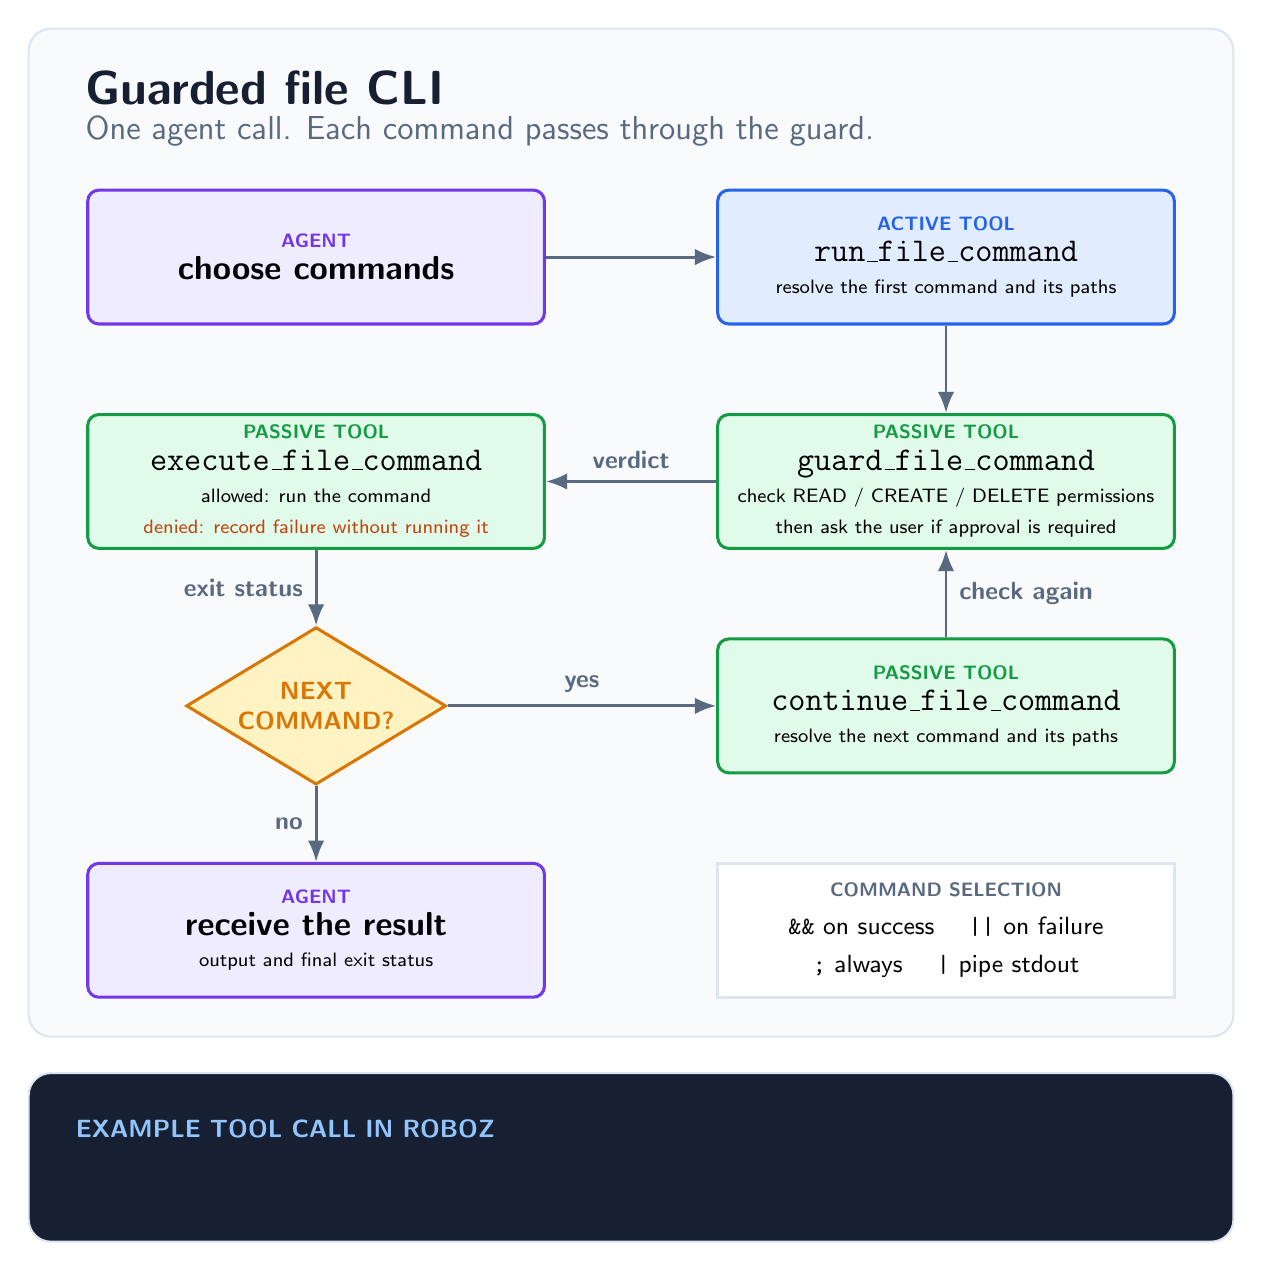
\begin{tikzpicture}[font=\sffamily]
  \begin{scope}[on background layer]
    \draw[draw=panelborder,fill=panel,line width=0.75pt,rounded corners=8pt]
      (-3.65,2.45) rectangle (11.65,-10.35);
  \end{scope}

  \node[anchor=west,font=\sffamily\bfseries\LARGE,text=ink] at (-3.05,1.7)
    {Guarded file CLI};
  \node[anchor=west,font=\sffamily\large,text=muted] at (-3.05,1.15)
    {One agent call. Each command passes through the guard.};

  \node[agent] (agent) at (0,-0.45) {
    {\scriptsize\bfseries\color{purple}AGENT}\\[-0.2mm]
    {\large\bfseries choose commands}
  };
  \node[tool] (entry) at (8,-0.45) {
    {\scriptsize\bfseries\color{blue}ACTIVE TOOL}\\[-0.2mm]
    {\large\bfseries\texttt{run\_file\_command}}\\[-0.2mm]
    {\scriptsize resolve the first command and its paths}
  };
  \node[passive] (guard) at (8,-3.3) {
    {\scriptsize\bfseries\color{green}PASSIVE TOOL}\\[-0.2mm]
    {\large\bfseries\texttt{guard\_file\_command}}\\[-0.2mm]
    {\scriptsize check READ / CREATE / DELETE permissions}\\[-0.2mm]
    {\scriptsize then ask the user if approval is required}
  };
  \node[passive] (execute) at (0,-3.3) {
    {\scriptsize\bfseries\color{green}PASSIVE TOOL}\\[-0.2mm]
    {\large\bfseries\texttt{execute\_file\_command}}\\[-0.2mm]
    {\scriptsize allowed: run the command}\\[-0.2mm]
    {\scriptsize\color{red}denied: record failure without running it}
  };
  \node[decision] (next) at (0,-6.15) {
    {\small\bfseries\color{amber}NEXT}\\[-0.3mm]
    {\small\bfseries\color{amber}COMMAND?}
  };
  \node[passive] (continuation) at (8,-6.15) {
    {\scriptsize\bfseries\color{green}PASSIVE TOOL}\\[-0.2mm]
    {\large\bfseries\texttt{continue\_file\_command}}\\[-0.2mm]
    {\scriptsize resolve the next command and its paths}
  };
  \node[agent] (resume) at (0,-9) {
    {\scriptsize\bfseries\color{purple}AGENT}\\[-0.2mm]
    {\large\bfseries receive the result}\\[-0.2mm]
    {\scriptsize output and final exit status}
  };
  \node[context] (operators) at (8,-9) {
    {\scriptsize\bfseries\color{muted}COMMAND SELECTION}\\[0.6mm]
    {\small\texttt{\&\&} on success \quad \texttt{||} on failure}\\[0.6mm]
    {\small\texttt{;} always \quad \texttt{|} pipe stdout}
  };

  \draw[flow] (agent.east) -- (entry.west);
  \draw[flow] (entry.south) -- (guard.north);
  \draw[flow] (guard.west) -- node[edge label,above=0.8mm] {verdict} (execute.east);
  \draw[flow] (execute.south) -- node[edge label,left=0.8mm] {exit status} (next.north);
  \draw[flow] (next.east) -- node[edge label,above=0.8mm] {yes} (continuation.west);
  \draw[flow] (continuation.north) -- node[edge label,right=0.8mm] {check again} (guard.south);
  \draw[flow] (next.south) -- node[edge label,left=0.8mm] {no} (resume.north);

  % Match the flow panel's left and right edges: -3.65 cm and 11.65 cm.
  \node[anchor=north,draw=panelborder,fill=ink,line width=0.75pt,
    rounded corners=8pt,text width=141mm,inner sep=6mm,align=left]
    at (4,-10.8) {
      {\sffamily\bfseries\small\color{codeblue}EXAMPLE TOOL CALL IN ROBOZ}\par
      \vspace{3mm}
      \usebox{\clijsonbox}
    };
\end{tikzpicture}
\end{document}
